\chapter{Entwicklungsprozess und Dokumentation}

Im folgenden wird ein Überblick über die verschiedenen verwendeten Technologien und Bibliotheken gegeben, der Entwicklungsprozess dargestellt und die Webapp selbst vorgestellt.

\section{Auswahl der Technologien und Bibliotheken}

Zu Beginn des Projektes habe ich mich viel mit Webdevelopment und -design im Allgemeinen beschäftigt: Entwicklungsprozesse, Designrichtlinien und -prinzipien z.B. für die richtige Verwendung von Farben, Bildern und Schrift, sowie Best Practices bei der Verwendung von HTML, CSS und Javascript (JS), oder bei Anfragen an das Backend einer Website. Außerdem habe ich passende Bibliotheken sowie Ressourcen für einige grafische Elemente wie Schriftarten und Symbole herausgesucht. 

\subsection{Javascript Framework - React}

Modernes Webdevelopment, gerade bei komplexeren Apps wie dieser, benutzt fast immer Javascript Frameworks mit zusätzlichen Funktionen, im Gegensatz zum klassischen Ansatz, der sich nur auf Javascript, HTML und CSS beschränkt. Hauptsächlich sind momentan die folgenden drei Frameworks in Verwendung:

\begin{itemize}
    \item \textbf{React}
    \begin{itemize}
        \item Von Facebook
        \item Großer Fokus auf Stabilität bei der Weiterentwicklung, Upgrade/Migration auf neuere Version am einfachsten
        \item Momentan am weitesten verbreitet und unterstützt => guter Support und Dokumentation von anderen Bibliotheken
        \item Minimalistischer als Angular (weniger Funktionen, kleiner) => einfacher zu lernen, braucht dafür allerdings zusätzliche Bibliotheken für einige Aufgaben, mit denen es sich aber leicht integrieren lässt
        \item Besser als Angular für sehr dynamische/interaktive Seiten (wie hier) geeignet
        \item Kann schneller als Angular sein, da es mit einer virtuellen Document Object Model (DOM) arbeitet anstatt die reale DOM zu verändern
    \end{itemize}

    \item \textbf{Angular}
    \begin{itemize}
        \item Von Google
        \item Relativ große und komplette Bibliothek, mehr ein Framework als eine Library wie React
        \item Fast so weit verbreitet wie React, die Verbreitung hat die letzten Jahre allerdings abgenommen
        \item Benutzt Typescript anstelle von Javascript
    \end{itemize}
    \item \textbf{Vue}
    \begin{itemize}
        \item Von keinem Unternehmen entwickelt oder unterstützt
        \item Am wenigsten verbreitet, wächst allerdings am schnellsten
        \item Am neuesten und noch nicht sehr weit verbreitet
    \end{itemize}
   
\end{itemize}


Bei diesem Projekt werden zur Anpassung der Trackingdaten sowie zum Erstellen von Diagrammen weitere Bibliotheken verwendet werden. Aufgrund der leichten Integration mit anderen Bibliotheken, der großen Flexibilität aufgrund des minimalistischeren Designs, sowie der großen Verbreitung und damit einhergehenden guten Supports und Dokumentation habe ich mich zur Nutzung von React entschieden.


\subsection{Andere Javascript Bibliotheken}

Neben React wurden für einige Funktionen noch andere Libraries eingebunden, unter anderem zum Zeichnen grafischer Objekte, zur einfachen Erzeugung von Diagrammen, Textfeldern und vorgefertigten React Komponenten.

\subsubsection{Fabric.js}\label{chapter:fabric}

Für den Tracking Editor wurde eine Library benötigt, um Bounding Boxes, Text, und Eckpunkte auf den einzelnen Frames des zu analysierenden Videos einzublenden. Nativ kann das auf einem HTML Canvas Elements ebenfalls passieren. Allerdings wäre das vergleichsweise umständlich, es können nur Pfade und Rechtecke verwendet werden und diese beispielsweise nicht verschoben werden, sondern nur gelöscht und an anderen Stelle neu gezeichnet. Daher habe ich für diese Projekt Fabric.js verwendet, die mehr Funktionen, grundlegende Animationen und eine einfachere Benutzung bereitstellt, ohne zu umfangreich oder unnötig komplex zu sein. Eine andere Alternative wäre Two.js gewesen, die allerdings mehr auf Animation ausgerichtet ist. Graphics.js kann ebenfalls einfache Formen zeichnen, diese können allerdings nicht umherbewegt werden.

\subsubsection{Chart.js}

Für die Diagramme in der Analyse Sektion der Webapp habe ich Chart.js verwendet. Es unterstützt acht verschiedene Arten von Diagrammen, mit ansprechendem, modernen flachen Design, die bereits standardmäßig mit einigen simplen Animation ausgestattet sind. Anderen Alternativen sind oft umfangreicher, wurden aber nicht benötigt. Vor allem D3.js ist sehr mächtig, hat dafür aber eine sehr steile Lernkurve und keine vorgefertigten Diagramme. Plotly.js ist mit D3 gebaut und hat einige vorgefertigte Darstellungen für wissenschaftliche Diagramme.

\subsubsection{React-Edit-Text}

React-Edit-Text stellt vorgefertigte Textfeld Komponenten bereit, mit denen Text angezeigt und direkt bearbeitet werden kann, wobei die Größe des Textfeldes automatisch angepasst wird. Leider scheint keine vergleichbar einfach zu benutzende und prinzipiell gut funktionierende Bibliothek zu existieren. React-Edit-Text hat leider einige kleine Bugs bzw. unerwünschtes Verhalten, z.B. wird beim Bearbeiten des Textes teilweise die Breite des Textfeldes (und damit oft des umliegenden Containers) verändert. Hier könnten durch Lösung mit Hilfe anderer Textfeldkomponenten einige kleine kosmetische Verbesserungen an der Webapp erreicht werden.

\subsubsection{Google Material UI Components}

Einige Komponenten wären nur mit viel Aufwand selbst umsetzbar, gerade wenn diese Animationen beinhalten, wie zum Beispiel Schalter, Buttons oder Dropdown Menüs. Für solche Komponenten eignen sich die vorgefertigten und individuell anpassbaren vorgefertigten Komponenten von Googles Material UI (MUI) sehr gut. Sie stellen ein einheitliches Design inklusive einigen Animationen bereit. In diesem Frontend habe ich die meisten Komponenten selbst erstellt, für einige einzelne Elemente allerdings auf MUI zurückgegriffen. Aufgrund nicht immer klarer Dokumentation ist die Arbeit mit MUI am Anfang oft recht aufwändig, sobald die einzelnen Komponenten allerdings bereits benutzt wurden, können diese sehr einfach an anderen Stellen wiederverwendet und angepasst werden. Die API ist jedoch stark darauf ausgelegt, dass die komplette Anwendung mit MUI erstellt wird und meist das Standard Styling beibehalten wird. In dieser Webapp habe ich deshalb oft MUI Eigenschaften lediglich in CSS überschrieben, um das gesamte Styling möglichst einheitlich zu halten, anstatt explizit ein eigenes MUI Thema zu erstellen, dass dann nur für die MUI Komponenten wirksam ist. Insgesamt ist MUI zwar teilweise unintuitiv und umständlich zu benutzen bzw. anzupassen, die Anpassbarkeit sowie das bekannte, verbreitete und professionelle wirkende Google Design spricht allerdings trotzdem sehr für die Benutzung. 

\subsection{Provider für Icons und Schriftarten}


\subsubsection{Icon Provider - Svgbox \& Fontawesome} \label{icons}

Als Service/Website zur Bereitstellung von Icons/Symbolen wie Home, Play, Delete etc. wurde wo möglich der ``Material'' Stil von SVGBox (\url{www.svgbox.net}) genutzt. Es stellt mit Abstand die größte Auswahl an Icons zur Verfügung und beinhaltet diese in verschiedenen Ausführungen. Bei einigen Icons wurde auf Fontawesome (\url{www.fontawesome.com}) zurückgegriffen, z.B. da die dort verfügbaren Symbole designtechnisch passender oder bei SVGbox nicht vorhanden waren. Alternative Quellen wären Bootstraps Glyphicons (\url{www.getbootstrap.com/docs/3.3/components/}), welche allerdings nur sehr wenige (250) Symbole bereitstellt, die teilweise weniger modern aussehen und mithilfe eines <span> HTML Elementes eingefügt werden, was den Code etwas weniger lesbar und übersichtlich macht. Auch Google stellt Icons im Material Design unter \url{www.material.io/resources/icons} bereit. Diese Symbole sind am meisten konfigurierbar was Größe, Design und Farbgebung anbelangt, sehen sehr modern aus, aber haben mit 750 Icons auch nur eine eingeschränkte Auswahl bei der einige benötigte Symbole nicht auffindbar waren. Alle diese Anbieter lassen es zu, Icons als Scalable Vector Graphic (SVG) Datei herunterzuladen und in der App selbst zur Verfügung zu stellen oder via  Content Delivery Network (CDN) direkt über die Server der Anbieter zu laden und so in der Webapp zur Verfügung zu stellen. Außerdem können alle genannten Icons frei verwendet werden, bei den Glyphicons wird allerdings um eine Quellenangabe gebeten.
\\
\\
Alle in dieser Webapp verwendeten Fontawesome Inhalte werden per CDN geladen (wie in \linebreak\url{www.fontawesome.com/how-to-use/on-the-web/using-with/react/} beschrieben). Dadurch wird die vom Backend dieser Webapp benötigte Bandbreite reduziert und auf das CDN ausgelagert. Im Gegensatz dazu werden alle SVGBox Symbole als SVG Dateien im \texttt{/src/icons} Ordner der Website abgelegt, sodass die Quelle der verwendeten Symbole immer klar ersichtlich ist.

\subsubsection{Schriftarten Provider - Googlefonts}

Für die Schriftarten wurde auf Google Fonts (\url{www.fonts.google.com}) zurückgegriffen, da dies den Standard zur Bereitstellung von Schrift darstellt. Die beiden verwendeten Schriftarten sind in src/fonts abgelegt. 


\section{Codestruktur und Namenskonventionen}

Generell folgt der Code den in der Javascript bzw. React Entwicklung gängigen Konventionen:
\begin{itemize}
    \item \textbf{JS Klassennamen:} UpperCamelCase; Oft wurden Kindklassen nach dem Schema ElternkomponentKindKind... benannt.
    \item \textbf{JS Dateien:} Gleicher Name wie enthaltene Klasse
    \item \textbf{JS Methoden und Variablen:} lowerCamelCase
    \item \textbf{CSS Dateien}: Gleicher Name wie die hierarchisch höchste JS Datei, die sie benutzt; Kindklassen / -dateien benutzen meist die CSS Dateien der Eltern, um alle Style Regeln für eine Seite möglichst in einer Datei zu sammeln.
    \item \textbf{CSS Klassen:} Jede React Komponente hat ihren Namen/JS Klasse auch als HTML Klassennamen zugewiesen. Innere Elemente sind meist nach dem Schema KlassennameElementSubelement... benannt. Bei tiefen Verschachtelung, nur für das Styling notwendigen Containern und generell wo es der Lesbarkeit und Übersichtlichkeit zuträglich erschien, wurden hier einige Ausnahmen gemacht. Generische Klassen, die sich auf Eigenschaften anstatt die eindeutige Definition eines Objektes beziehen, sind in lower-dashed-case wie in CSS üblich.
\end{itemize}

Die App wurde mittels dem create-react-app Befehl/Skript erstellt und folgt der Standard React App Struktur. Alle im Rahmen dieses IDPs verwendeten Dateien, Daten und Dokumentation befinden sich im zur Entwicklung verwendeten GitLab Repository (\url{https://gitlab.lrz.de/ga38vud/saasfrontend}) unter dem \texttt{frontend} Ordner. Wie die notwedingen Bibliotheken zu installieren sind und die App auszuführen ist, ist in der dem Code beigefügten Readme Datei dokumentiert. Alle verwendeten Pakete und Versionen sind in der \texttt{package.json} Datei aufgeführt. Der \texttt{public} Ordner beinhaltet die Favicons (die kleinen Symbole, die der Webbrowser oben im Tab der Webapp anzeigt) und alle notwendigen Metadaten und die \texttt{index.html} Datei, die das ursprüngliche HTML Dokument für eine React App ist, in die alle anderen Inhalte eingefügt werden. Die Favicons wurden mit der Website \url{https://favicon.io/favicon-converter/} formatiert und in das passende Format gebracht. Als Motiv diente ein Screenshot der Startseite der Webapp, bei der der Game Tracker Schriftzug zu GT abgeändert wurde.
\\
Der restliche Sourcecode der Applikation befindet sich im \texttt{src} Ordner. Alle sich dort nicht in weiteren Unterordnern befindlichen Dateien bis auf die CSS Dateien und \texttt{App.js} sollten bei der Weiterentwicklung keine weiteren Änderungen erfordern und wurden auch nach der automatischen Erzeugung durch create-react-app nicht weiter geändert. Im Folgenden sind alle relevanten Elemente in \texttt{/src} aufgeführt:

\begin{itemize}
    \item \textbf{index.css}: Grundlegende CSS Eigenschaften für das gesamte Projekt, z.B. Schriftarten
    \item \textbf{App.js}: Handelt das Routing und fügt je nach aktueller URL/Pfad die passenden React Komponenten zur Darstellung der einzelnen Seiten ein
    \item \textbf{/components}: Alle selbst erstellten React Komponenten, die in \texttt{App.js} benutzt wurden
    \begin{itemize}
        \item \textbf{/layout}: Beinhaltet alle auf mehreren Seiten verwendeten Layout Komponenten, in diesem Fall nur den Header und die zugehörige CSS Datei
        \item \textbf{/pages}: Alle React Komponenten, die zu einzelnen Unterseiten der App gehören, bei mehrern Dateien jeweils in eigenem Unterordner pro Unterseite mit allen verwendeten Komponenten und CSS Dateien
    \end{itemize}

    \item \textbf{/data/}: Alle in der Applikation verwendeten Daten, die eigentlich vom Backend bereitgestellt werden sollen. Da bis jetzt noch kein Backend existiert, wurden Bilddateien hier abgelegt und \texttt{.json} Dateien erstellt, die beispielhafte Antworten des Backends darstellen und deren Inhalte in der Webapp angezeigt werden. Alle Bilder und \texttt{tracking\_data.json} wurden mir zur Entwicklung vom Lehrstuhl bereitgestellt, die restlichen Dateien wurden selbst mit beispielhaften Daten manuell erzeugt.

    \item \textbf{/fonts/}: Die Schriftartdateien aller verwendeten, nicht standardmäßig in Webbrowsern vorhandenen Schriftarten.

    \item \textbf{/icons/}: Symbole im SVG Format, die in der App verwendet werden. Alle hier abgelegten Symbole stammen von SVGBox (siehe \ref{icons}).

    \item \textbf{/pictures/}: Alle in der Webapp zu gestalterischen Zwecken verwendeten Bilder (also alle, die keine durch die Applikation zu verarbeitenden Daten sind und deshalb in \texttt{/data} abgelegt werden).

    \begin{itemize}
        \item \textbf{dark\_football\_field.jpg}: Wird auf der Startseite als Hintergrundbild verwendet. Es handelt sich hier um ein zur freien Verwendung und Bearbeitung zur Verfügung gestellten Stockfoto, das mit der Bildbearbeitungssoftware Gimp bearbeitet wurde. Das Bild wurde durch ein Overlay dunkler gemacht, einige Spieler an störenden Position wurden wegretouchiert und die Dateigröße wurde für ein schnelleres Laden reduziert.
        \item \textbf{green\_grass\_texture\_512x512.png}: Ein Gras Texturbild (also ein Bild, das ohne sichtbare Übergänge beliebig nebeneinander wiederholt werden kann), das als optionaler Hintergrund in den Unterseiten \texttt{/games} und \texttt{/analysis/<id>} dient (siehe Kapitel \ref{chapter:file-overview} und \ref{chapter:analysis}). Momentan ist der entsprechende Code zu Gunsten eines grauen Hintergrunds auskommentiert.
    \end{itemize}
\end{itemize}

\section{Überblick über die Webapp}

Im Folgenden wird zuerst ein schematischer Überblick über die Webapp mit ihren einzelnen Unterseiten wie in \autoref{fig:structure-overview} dargestellt gegeben und diese dann in den jeweiligen Unterkapiteln näher erläutert.

\begin{figure}[h]
 \centering
 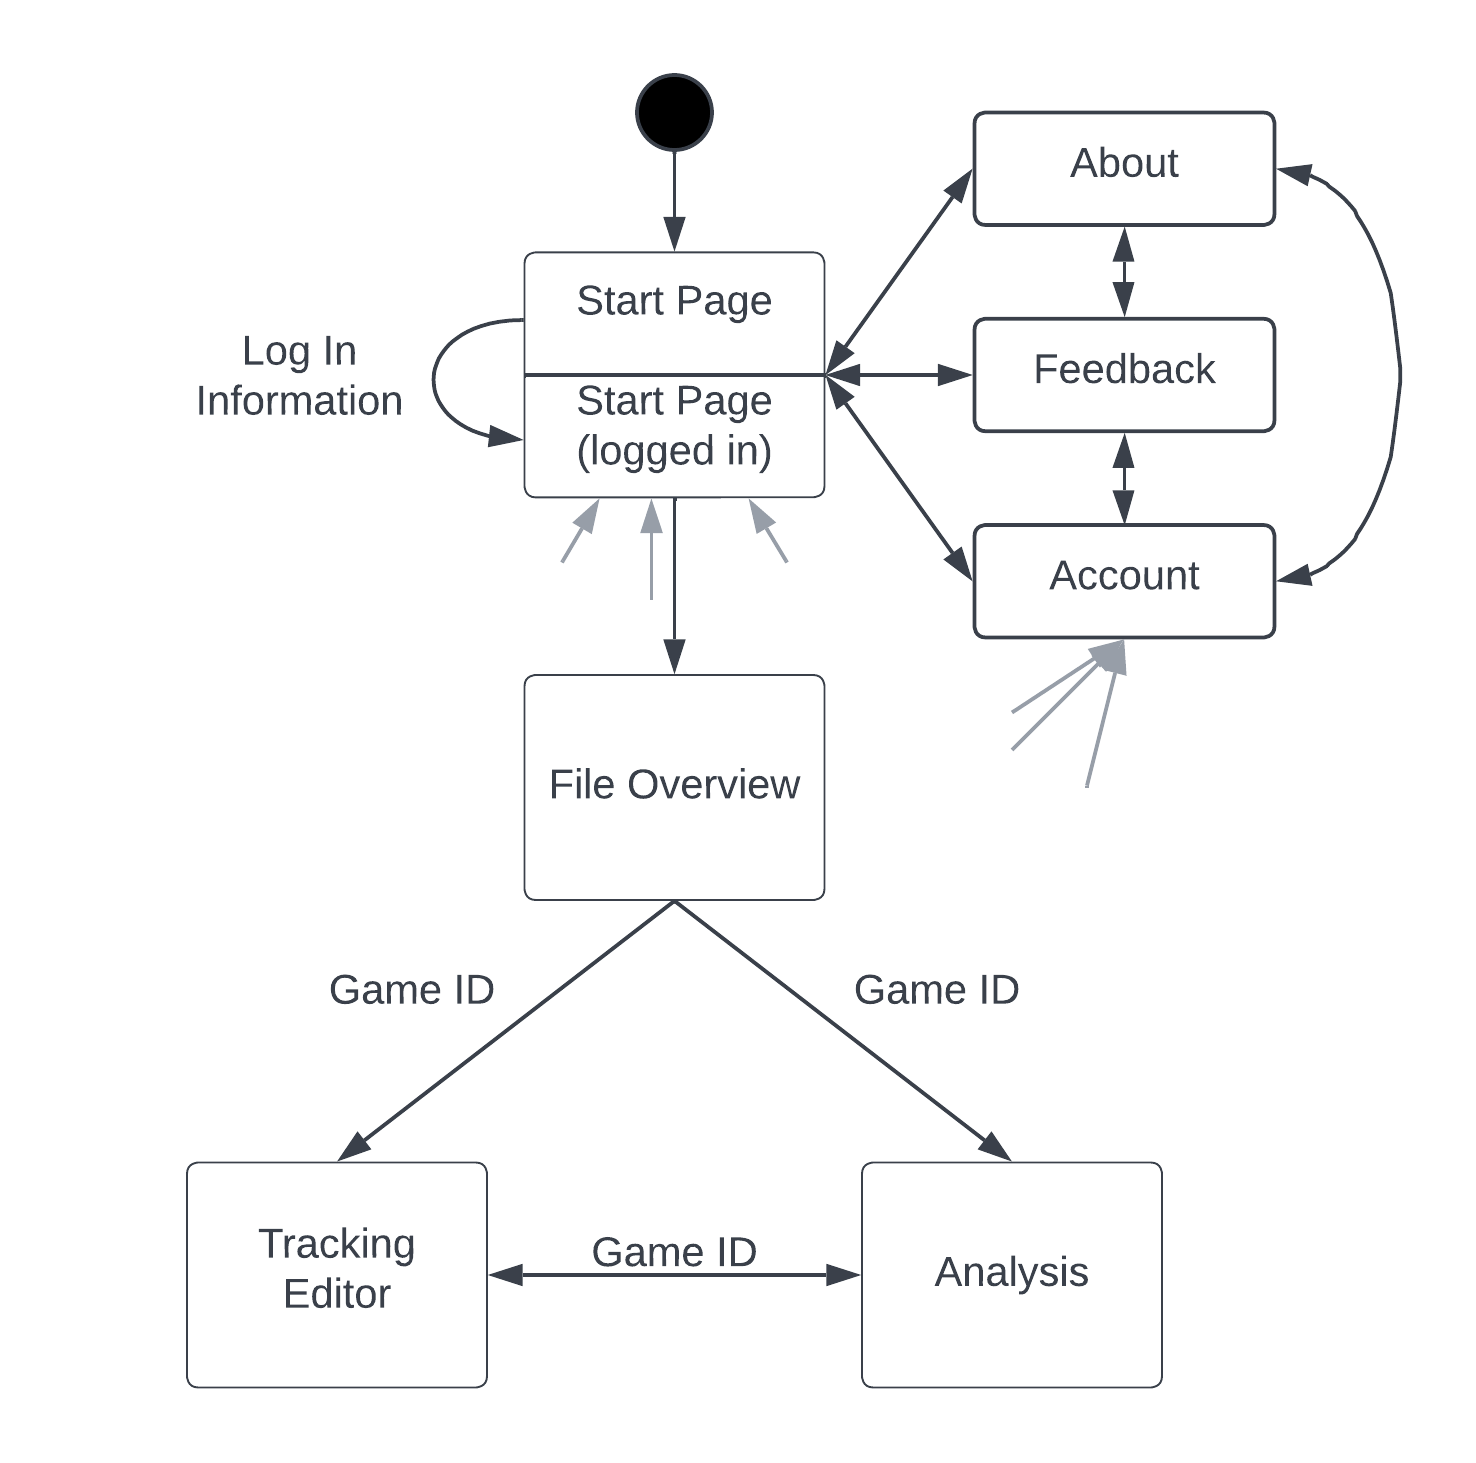
\includegraphics{images/Diagram_Website_Global_Structure.png}
 \caption{Die Strukture der Webapp mit ihren einzelnen Unterseiten. Die grau angedeuteten Pfeile stellen dar, dass die entsprechenden Seiten von jeder anderer Stelle der Applikation über die Navigationskopfleiste (Header) erreicht werden können. Der schwarze Kreis ist der Beginn des Diagramms, die Startseite wird zuerst aufgerufen.}
 \label{fig:structure-overview}
\end{figure}

Die About, Feedback und Account Seiten wurden nur mit einer einzelnen Überschrift befüllt und für das zukünftige Ausfüllen offen gelassen. Die Userverwaltung und damit der Login und die Account Übersichtsseite hängen stark vom Backend ab. Einige Backend Technologien, z.B. von Amazon Web Services, bieten bereits einfach zu integrierende Loginseiten, die hier genutzt werden könnten. Generell läuft die Benutzung der Webapp so ab, dass der Benutzer nach dem Login auf die FileOverview Seite geht und dort ein Video eines Spiels hochlädt oder ein vorhandenes aussucht. Für das hochgeladene oder vorhandene Video kann er dann den TrackingEditor oder die Analyse öffnen. Im Tracking Editor sieht er die nach dem Upload automatisch durch das zukünftige Backend generierten Trackingdaten. Die Spieler und Ecken des Spielfeldes sind mit Bounding Boxen bzw. Punkten versehen. Diese Daten sind idealerweise bereits korrekt, können aber hier kontrolliert und ggf. korrigiert werden. In der Analyse Seite kann er selbst verschiedene Arten von Diagrammen und Subsets von Teams oder Spielern auswählen so eine beliebige Auswahl an Analysebausteinen generieren. Er kann mithilfe der Links im Header auch direkt zwischen dem Tracking Editor und der Analyse für ein Video hin und her springen sowie stets zurück zur Startseite oder seiner Profilseite (Account) navigieren. \\
Das spätere Backend sollte nach Bearbeitung der Tracking Daten gegebenenfalls die Inhalte der Analyse neu aus den aktualisierten Daten generieren.

\subsection{Startseite}

Die Startseite wurde als simple Landing Page gestaltet, mit einem Header zur Navigation, dem Titel ``Game Tracker'', der natürlich in Zukunft noch angepasst werden kann, sowie einigen Buttons für alle benötigten Operationen. Der Code für den Header, der hier und auf allen anderen Seiten angezeigt wird, befindet sich in \texttt{/src/components/layout/}. Die About, Feedback und Profil (das Benutzersymbol oben rechts) Links führen den Nutzer auf die jeweilige Unterseite, die momentan nur aus einem HTML Header mit dem Titel der Seite besteht. Diese sind in der Datei \texttt{/src/App.js} zu finden und können zum Weiterentwickeln in eigene Komponenten ausgelagert werden, analog z.B. zu der Startseiten Komponente \texttt{Start}, die sich in der gleichnamigen Datei unter \texttt{/src/components/pages/} befindet.
\\
Welche Art von Header angezeigt wird (die große Version auf der Startseite oder die kleinere auf den anderen Seiten) und wie dieser beim Laden der Seite animiert wird, ist in \texttt{/src/App.js} geregelt. Welche Links im Header angezeigt werden, regelt dieser selbst, indem er die aktuelle URL ausliest. \autoref{fig:start-page} zeigt die Startseite im Zustand mit einem eingeloggtem Benutzer. Da das Backend momentan noch fehlt, wird dies über eine auf \texttt{true} gesetzte Variable \texttt{loggedIn} im React state der Start Komponente definiert. Wie bei allen für die Integration des Backends notwendigen Änderungen wurde ein auskommentiertes und mit einem ``TODO BACKEND ...'' Kommentar versehenes Stück Code ergänzt, das eine beispielhafte Backend Anfrage und wie deren Antwort weiterverarbeitet werden sollte demonstriert. Eine Übersicht über die notwendigen Funktionen und das Vorgehen bei der Integration des Backends findet sich in \autoref{chapter:backend-integration}.\\

\begin{figure}[h]
 \centering
 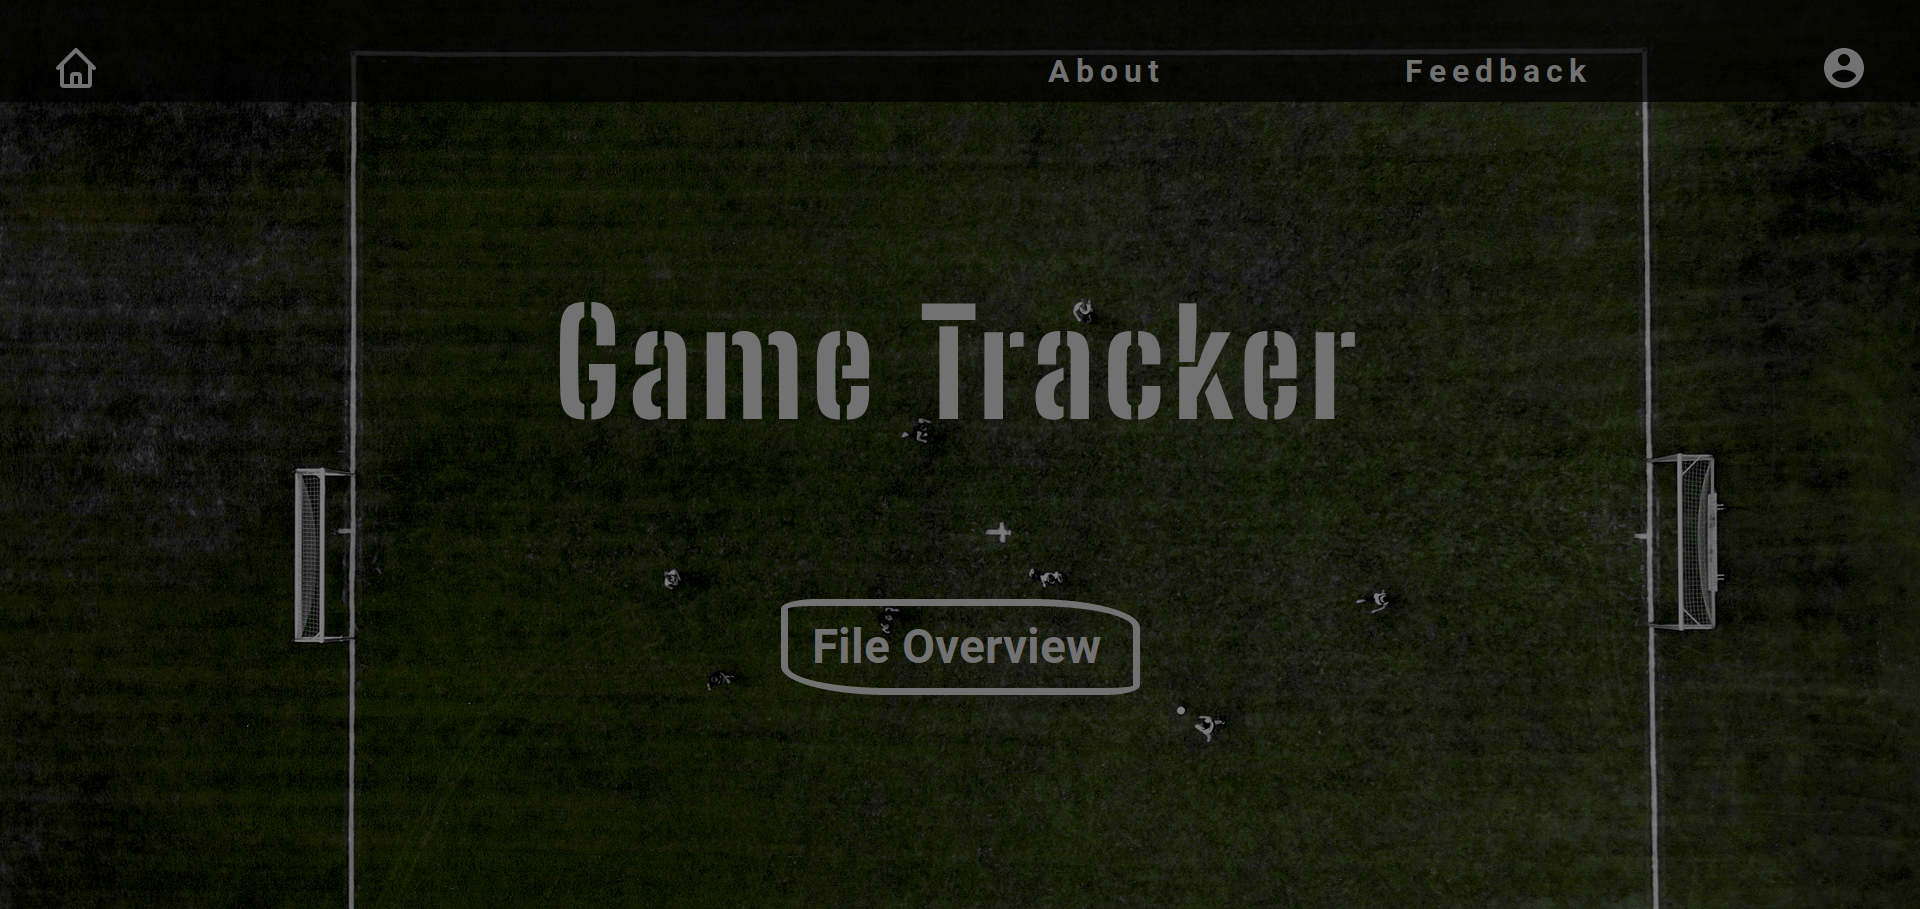
\includegraphics[width=17cm]{images/Start_page.png}
 \caption{Die Startseite der Webapp.}
 \label{fig:start-page}
\end{figure}

Falls der Nutzer nicht eingeloggt ist (kann momentan durch manuelles Setzen der Variable in der \texttt{componentDidMount()} Funktion auf \texttt{false} simuliert werden), dann wird der ``File Overview'' Button nicht angezeigt, da ja kein Nutzer eingeloggt ist, der schon Daten hochgeladen hat und diese ansehen kann. Stattdessen werden die Buttons Demo, Log In und Register angezeigt. Die Idee hinter der Demo Funktion war, dass der Nutzer bereits ohne Registrierung und Hochladen eines eigenen Videos, was eine große Hürde für das erstmalige Ausprobieren eine Webapp darstellt, bereits einige Funktionen testen kann. Deshalb wird er auf eine Instanz des Tracking Editors weitergeleitet, wo er diesen anhand von Beispieldaten ausprobieren kann. Momentan werden dazu noch die in \texttt{/src/data/} abgelegten Beispieldaten verwendet, die aufgrund des fehlenden Backends ebenso noch von dem normalen Tracking Editor für eingeloggte User verwendet werden. Soll diese Funktion beibehalten werden, sollten diese Daten ebenfalls vom Backend zur Verfügung gestellt werden können. Genauso wäre es möglich, die beispielhaft manuell erzeugten Daten, die in der Analyse Seite angezeigt werden, als Demo verfügbar zu machen. Dafür müsste die App noch entsprechen erweitert werden, was allerdings mit wenig Aufwand möglich wäre.



\subsection{Übersicht über hochgeladene Videos}\label{chapter:file-overview}

Nach dem Einloggen kann der Nutzer dem File Overview Button folgen, um unter dem URL Pfad \texttt{/games} auf eine Übersichtsseite aller seiner hochgeladenen Videos zu kommen. Diese ist in \autoref{fig:file-overview} zu sehen. \\


\begin{figure}[h]
 \centering
 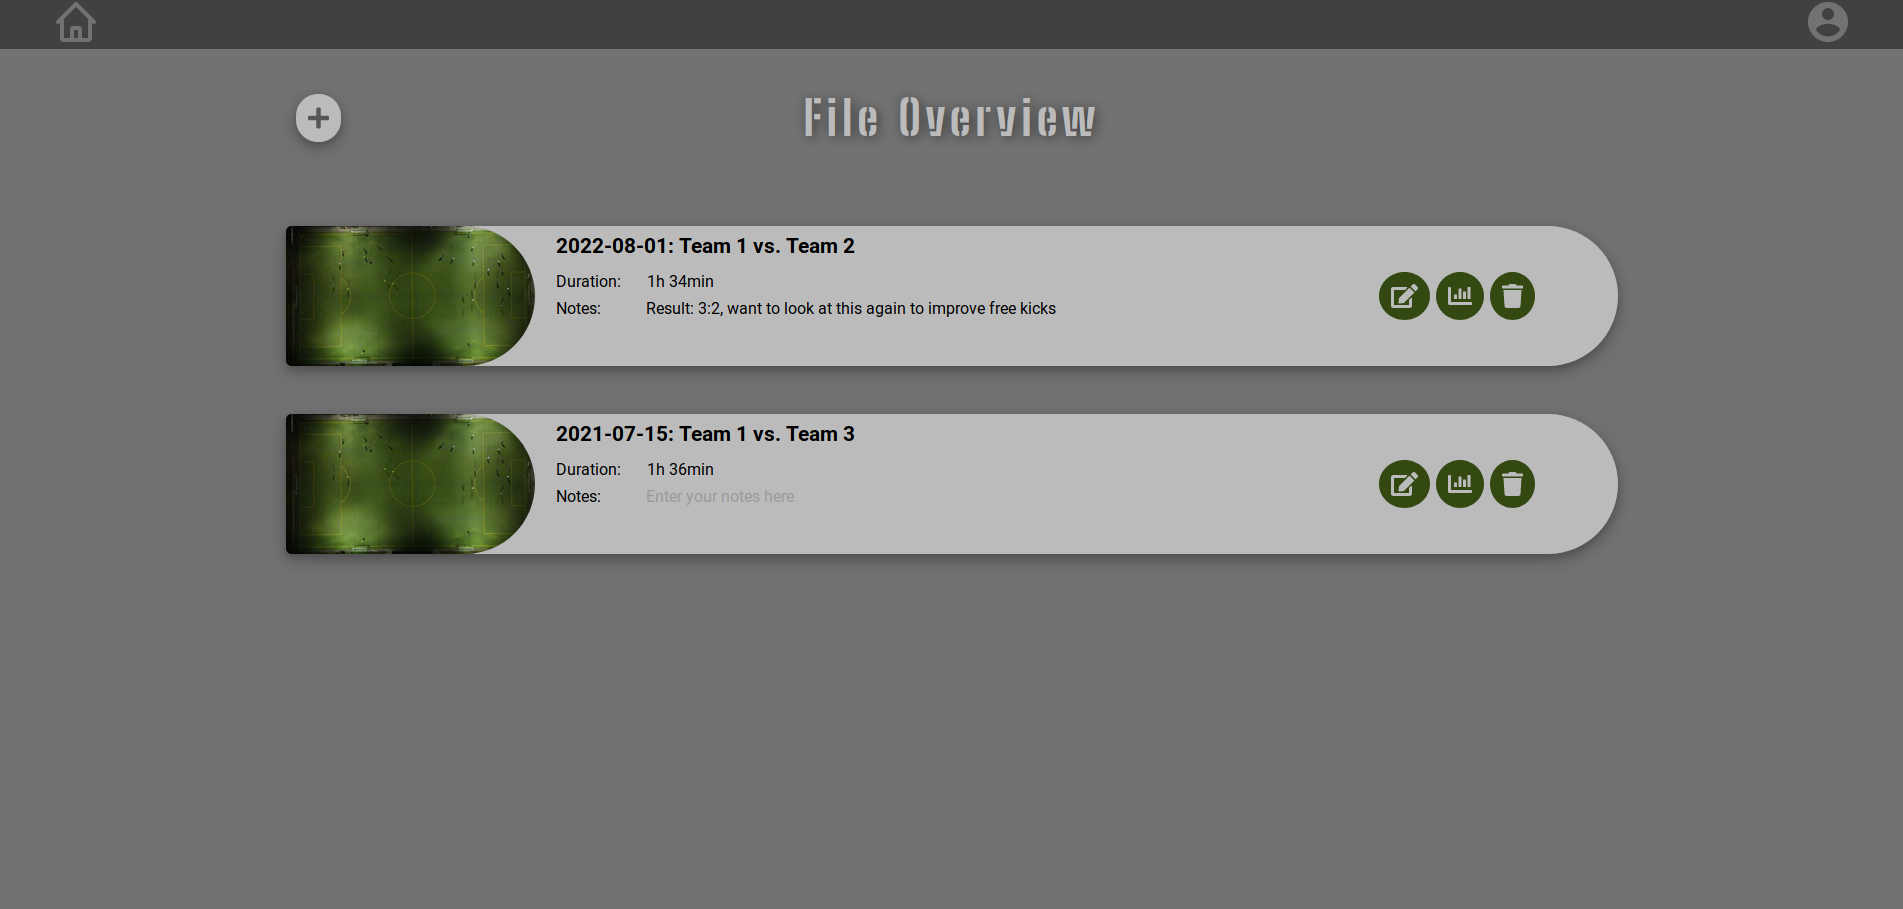
\includegraphics[width=17cm]{images/File_overview.png}
 \caption{Die Übersichtsseite über alle vom aktuellen Nutzer hochgeladene, analysierbare Videos.}
 \label{fig:file-overview}
\end{figure}

% Long Link below (\texttt{/src/components/pages/ fileOverview/fileOverview.js}) has a space so the line breaks
Der Plus Button links neben der Überschrift dient dem Upload neuer Videos. Bei einem Klick startet eine Animation, bei der sich der Button verbreitert, das Plus Symbol sich um 45° dreht und zu einem X bzw. Abbrechen Button wird und eine Schaltfläche zur Auswahl eines hochzuladenen Videos erscheint. Aufgrund des fehlenden Backends wird anstatt das Video hochzuladen allerdings nur eine kurze Bestätigungsmeldung angezeigt. Sobald ein Backend vorhanden ist, sollte wie im Code mit einem ``TODO BACKEND ...'' Kommentar vermerkt, in der \texttt{fileHandler()} Funktion in der Datei \texttt{/src/components/pages/ fileOverview/fileOverview.js} dieses für den Upload des Videos aufgerufen werden. Andere solche Kommentare zeigen, wo das Backend bei Änderungen der Videonamen oder Notizen, beim Löschen von Videos oder für das Laden der vorhandenen Videos aufgerufen werden muss.  Momentan werden die im Bild sichtbaren Einträge für die vorhandenen Videos aus der beispielhaften Backendantwort in \texttt{/src/data/videofiles.json} erzeugt. Die fileOverview Komponente in der gleichnamigen Datei liest diese aus und erstellt für jeden Eintrag eine Instanz der FileListItem Komponente. Der Code für diese Komponenten ist ebenfalls in der gleichnamigen Datei im \texttt{fileOverview} Ordner zu finden. Beide Komponenten importieren die \texttt{fileOverview.css} Datei, die das Styling für die gesamte Seite (mit Ausnahme des Headers) übernimmt. Die \texttt{FileListItem} Komponenten sind die hellgrau hinterlegten Listeneinträge, die in \autoref{fig:file-overview} zu sehen sind. Diese zeigen links einen Thumbnail des Videos, den Titel und Dauer des Videos sowie ein Feld für Notizen. Titel und Notizen können durch den Nutzer bearbeitet werden. Ganz rechts befinden sich drei grüne Buttons zum Bearbeiten der Spielererkennung/Trackingdaten, Öffnen oder Erstellen der Analyse und zum Löschen der jeweiligen Datei. Der Button ganz links öffnet den Tracking Editor, wobei die Id des jeweiligen Videos in der URL übergeben wird. Wird beispielsweise für das erste Video mit der Id 1 dieser Button angeklickt, wird der Nutzer zur Subseite \texttt{/trackingEditor/1} weitergeleitet und sieht den im folgenden Kapitel beschriebenen Tracking Editor, in dem Video 1 geöffnet ist. Da die Video Ids pro Nutzer vergeben werden, muss für die zukünftige Backendanfrage der aktuelle Benutzer bzw. seine Logindaten übergeben werden. So kann jeder Nutzer nur auf seine eigenen Videos zugreifen. Der mittlere der drei Buttons übergibt auf die gleiche Art die Video Id, nur öffnet er die im übernächsten Kapitel vorgestellte Analyse Seite anstatt des Tracking Editors. Der Button ganz rechts mit dem Abfalleimer Symbol fragt zuerst nach, ob das Video wirklich gelöscht werden soll und löscht es nach erfolgter Bestätigung durch den Nutzer.
\\
\\%Manually added linebreak in long link below: \texttt{/src/pictures/\linebreak green\_grass\_texture\_512x512.png
Im Verlaufe der Entwicklung habe ich außerdem mit einem alternativen Hintergrund für die File Overview Seite experimentiert. \autoref{fig:file-overview-alternative-background} zeigt diese alternative Grastextur (\texttt{/src/pictures/\linebreak green\_grass\_texture\_512x512.png} als Hintergrund. Um einen ausreichenden Kontrast zwischen dem Thumbnail der einzelnen Einträge und dem Hintergrund zu haben, habe ich die Höhe der Listeneinträge erhöht, um einen hellgrauen Rahmen um den Thumbnail zu erzeugen. Die Farbe des Headers könne ebenfalls noch zu einem helleren Grau geändert werden, um hier mehr Kontrast zu erzeugen. Allerdings habe ich den Hintergrund dann wieder zu Gunsten des einfarbigen grauen Hintergrundes verworfen, sodass der eigentliche Inhalt der Seite mehr im Vordergrund steht und um  längere Ladezeiten zu vermeiden. Außerdem könnte bei anderen Videos bzw. Thumbnails z.B. von einem roten Tenniscourt der Hintergrund farblich sowie thematisch unpassend sein. Der Code für den alternativen Hintergrund ist allerdings immer noch vorhanden und nur auskommentiert. In der \texttt{fileOverview.css} Datei sind zwei ``GRASS BACKGROUND'' Kommentare zu finden, die die notwendigen Änderungen beschreiben.

\begin{figure}[h]
 \centering
 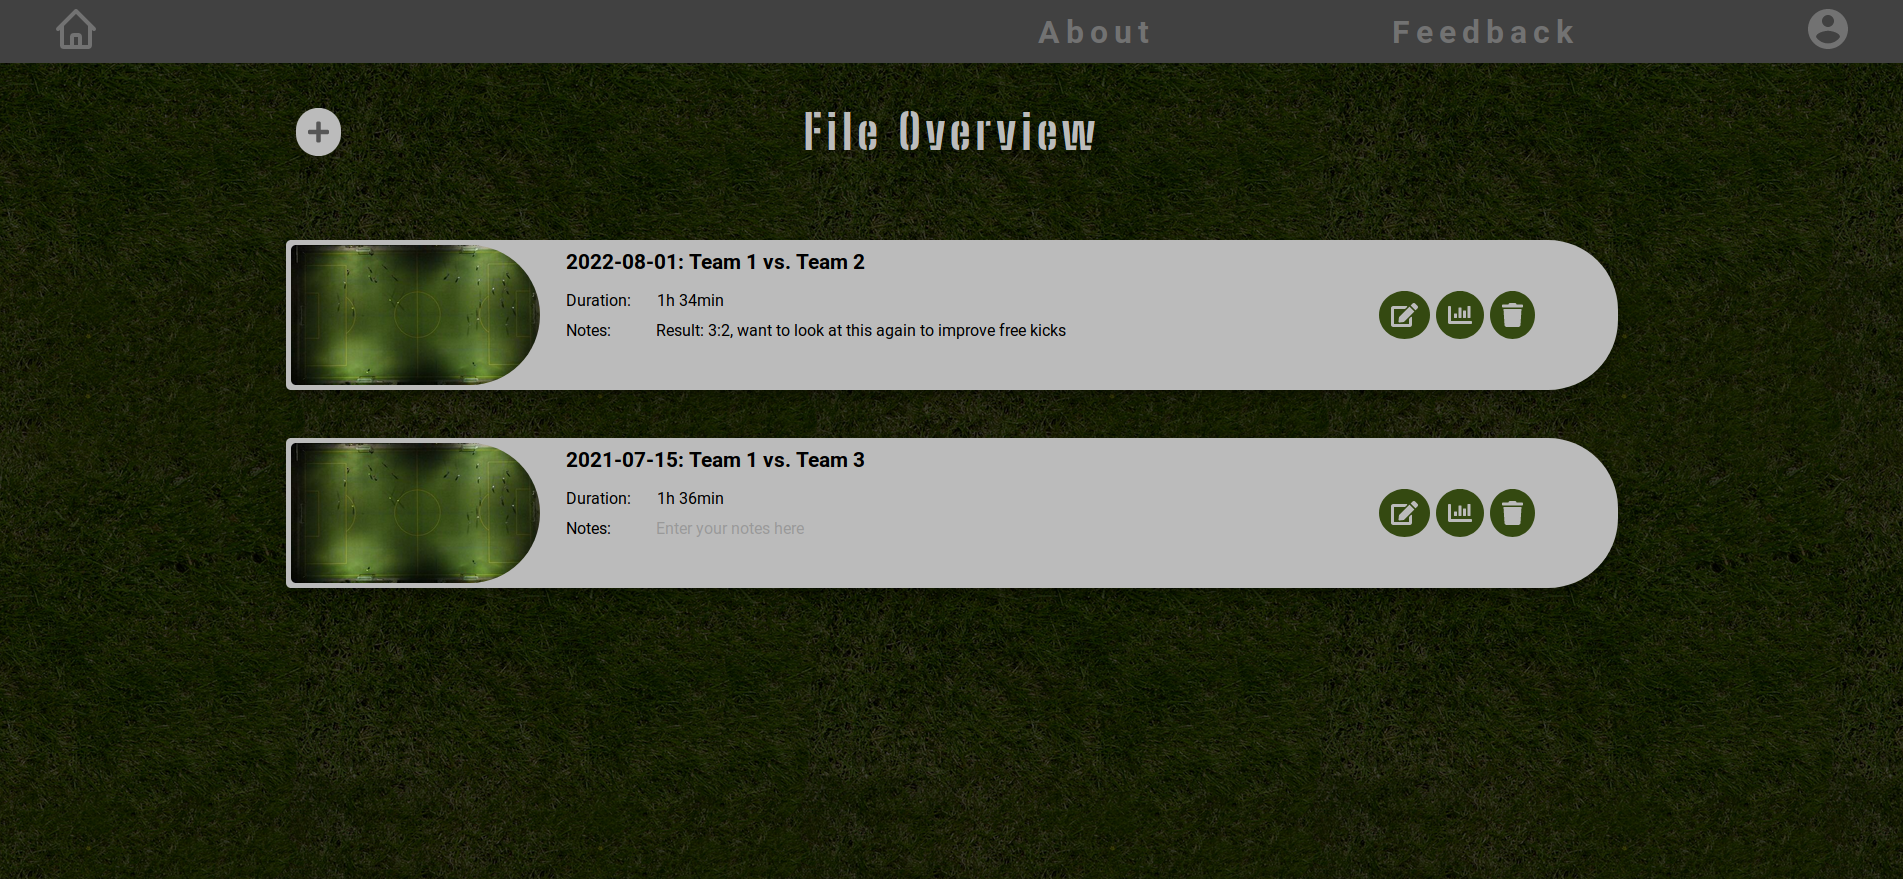
\includegraphics[width=17cm]{images/FileOverview_with_grass_background.png}
 \caption{Die Übersichtsseite mit alternativem Hintergrund.}
 \label{fig:file-overview-alternative-background}
\end{figure}

\subsection{Tracking Editor}

Unter der URL \texttt{/trackingEditor/<video\_id>} befindet sich der Tracking Editor, dargestellt in \autoref{fig:tracking-editor}. Aufgrund einem scheinbaren Bugs in React muss momentan manchmal die Seite im Browser manuell erneut geladen werden, damit der aktuelle Videoframe angezeigt wird. Sobald das Backend vorhanden ist, spielt dies allerdings sowieso keine Rolle mehr, da dann die Frames nicht mehr aus der lokalen JPG Datei geladen werden, sondern vom Backend kommen. Außerdem werden momentan für den Frame 0 keine Trackingdaten angezeigt, da die zur Verfügung gestellten Trackingdaten erst ab dem zweiten Frame (also Frame 1) beginnen, die Videoframes selbst aber mit Frame 0. Auf eine Anpassung, die die Frames erst ab Frame 1 beginnen lassen würde, habe ich verzichtet, da diese Änderung dann später für andere Daten wieder rückgängig gemacht werden müsste. Auch eine Verschiebung der Trackingdaten um einen Index scheint nicht vorzuliegen, da die Positionen der Bounding Boxes dann nicht mehr so gut mit den Spielen übereinstimmen würden.\\



Als Inspiration der Steuerung und des Designs wurde \url{www.cvat.org} herangezogen. Der Editor wird benutzt, um die durch die Algorithmen des Backends generierten Bounding Boxes um die erkannten Spieler und die Eckpunkte zu bearbeiten und/oder neue hinzuzufügen und die dazugehörigen Metadaten zu bearbeiten. Mit ihm können Bounding Boxes in der Größe verändert und umhergeschoben werden, indem diese direkt angeklickt werden. Die Eckpunkte des Spielfeldes können ebenfalls verschoben, aber nicht in der Größe geändert werden. Für diese Funktionen wurde die Bibliothek Fabric.js benutzt (siehe auch Kapitel \ref{chapter:fabric}), mit deren Hilfe Formen gezeichnet und manipuliert werden können. Fabric basiert auf einem HTML Canvas Element, bei dem hier der aktuelle Frame des Videos als Hintergrundbild gesetzt wird. Auf dieses Canvas werden dann Bounding Boxes, Ecken und ggf. die Metadaten wie Spielername etc. gezeichnet und mit entsprechenden Funktionen für das richtige Verhalten bei der Manipulation mit der Maus verknüpft. Die Basiskomponente, die auch den Code für dieses Canvas enthält, heißt \texttt{TrackingEditor} und findet sich in der gleichnamigen JS Datei unter \texttt{/src/components/pages/trackingEditor/}.\\

Die Trackingdaten werden momentan noch aus der \texttt{tracking\_data.json} Datei im \texttt{/src/data/} Ordner ausgelesen, müssten aber natürlich zukünftig vom Backend bereitgestellt werden. Diese JSON Datei ist die einzige, die für die Entwicklung vom Lehrstuhl zur Verfügung gestellt wurde und aus bereits vorhandenen Daten stammt und deshalb auch weitere, nicht verwendete Daten enthält. Allerdings werden nur die unter den JSON keys ``categories'' und ``annotations'' zu findenden Einträge verwendet. Die einzelnen Videoframes sind ebenfalls im gleichen Ordner zu finden.\\

Über dem Canvas und unter dem Header befindet sich die Navigationsleiste, die \texttt{Navbar} Komponente. Hier können mit den Pfeilen ganz links zukünftig Operationen rückgängig gemacht und wiederhergestellt werden. Dafür müssen die letzten Operationen im Backend gespeichert werden und bei einem Undo oder Redo Befehl an die Komponente gesendet werden, wo die gegebene Aktion dann ausgeführt werden muss. Rechts daneben befindet sich die Videosteuerung. Der Pfeil ganz links springt zum ersten Frame, der doppelte Pfeil spring zehn Frames zurück und der einfache Pfeil springt einen Frame zurück. Der Play Button lässt das Video alle paar Sekunden den nächsten Frame und die dazugehörigen Trackingdaten laden. Die Pfeile rechts davon sind analog zu den linken, nur spulen sie das Video vor anstatt zurück. Der Slider rechts von der Videosteuerung dient zur direkten Auswahl des Frames, genau wie das Auswahlfeld mit den Pfeilen direkt daneben. Slider und Auswahlfeld sind eine eigene, \texttt{Slider} genannte Subkomponente. Der Schalter rechts daneben mit der Bezeichnung ``Color by Teams'' kann in die Aus Position gebracht werden, um jeden Spieler in einer eigenen, zufällig generierten Farbe (die Farbe wird später vom Backend bereitgestellt) einzufärben, anstatt alle Spieler eines Teams mit der gleichen Farbe zu versehen. So kann schneller erkannt werden, welcher Spieler in der Liste rechts mit welcher Bounding Box auf dem Canvas korrespondiert. Als letztes Element befindet sich in der \texttt{Navbar} ein Dropdown Menü ``Label Visibility'', das einige Optionen zur Sichtbarkeit der Labels, also der Metadaten der einzelnen Bounding Boxes, zur Verfügung stellt. In \autoref{fig:tracking-editor} werden diese immer nur für die aktuell ausgewählte Box angezeigt. \\

Ganz rechts befindet sich die \texttt{TrackList} Komponente, die die einzelnen auf dem Canvas eingezeichneten Elemente auflistet. In den oberen Tabs kann zwischen den Spielern, Ecken und Teams umgeschaltet werden. Der oberste Eintrag der Liste mit dem Plussymbol ist die \texttt{TrackListItemAdd} Komponente und dient zum Hinzufügen von neuen Spielern bzw. Teams/Gruppen oder Ecken, je nachdem welche dieser Klassen in den Tabs gerade ausgewählt ist. Darunter befindet sich je nachdem, ob der Tab Players, Corners oder Groups ausgewählt ist, eine Liste mit \texttt{TrackListItemPlayer}, \texttt{TrackListItemCorner} oder \texttt{TrackListItemGroup} Komponenten. Alle diese Komponenten beinhalten einen veränderbaren Namen (außer die Ecken) sowie einen Löschbutton, der nach einer Bestätigung durch den Nutzer das jeweilige Element aus der Liste, dem Canvas und zukünftig dem Backend löscht. In \autoref{fig:tracking-editor} werden gerade die Spieler angezeigt, die einige weiteren Funktionen anbieten. Der Button mit der Taschenlampe direkt neben dem Namen startet eine Blink-Animation der Bounding Box. Diese wird auch beim Hinzufügen eines neuen Spielers für die neue Box ausgeführt und dient dazu, leicht die Position des zu dem Listeneintrag gehörenden Spielers auf dem Canvas zu sehen. Daneben befindet sich der Lösch Button und weiter der Button mit zwei Pfeilen, mit dem Spieler vertauscht werden können. Bei dem Generieren der Tracking Daten kann es vorkommen, das zwei Spieler vertauscht werden und die Bounding Boxes mit dem jeweils falschen Spieler assoziiert werden. Um diesen Fehler zu beheben, können mit dieser im Code ``swap'' genannten Funktion die beiden Bounding Boxes getauscht werden. Beim Klick auf den Button öffnet sich in einer Animation ein den Listeneintrag verbergendes Overlay, in dem der Tauschpartner ausgewählt und der Tausch bestätigt werden kann. Ganz rechts befindet sich schließlich ein Dropdown Menü, mit dem das dem Spieler zugeordnete Team verändert werden kann. \\

\begin{figure}[h]
 \centering
 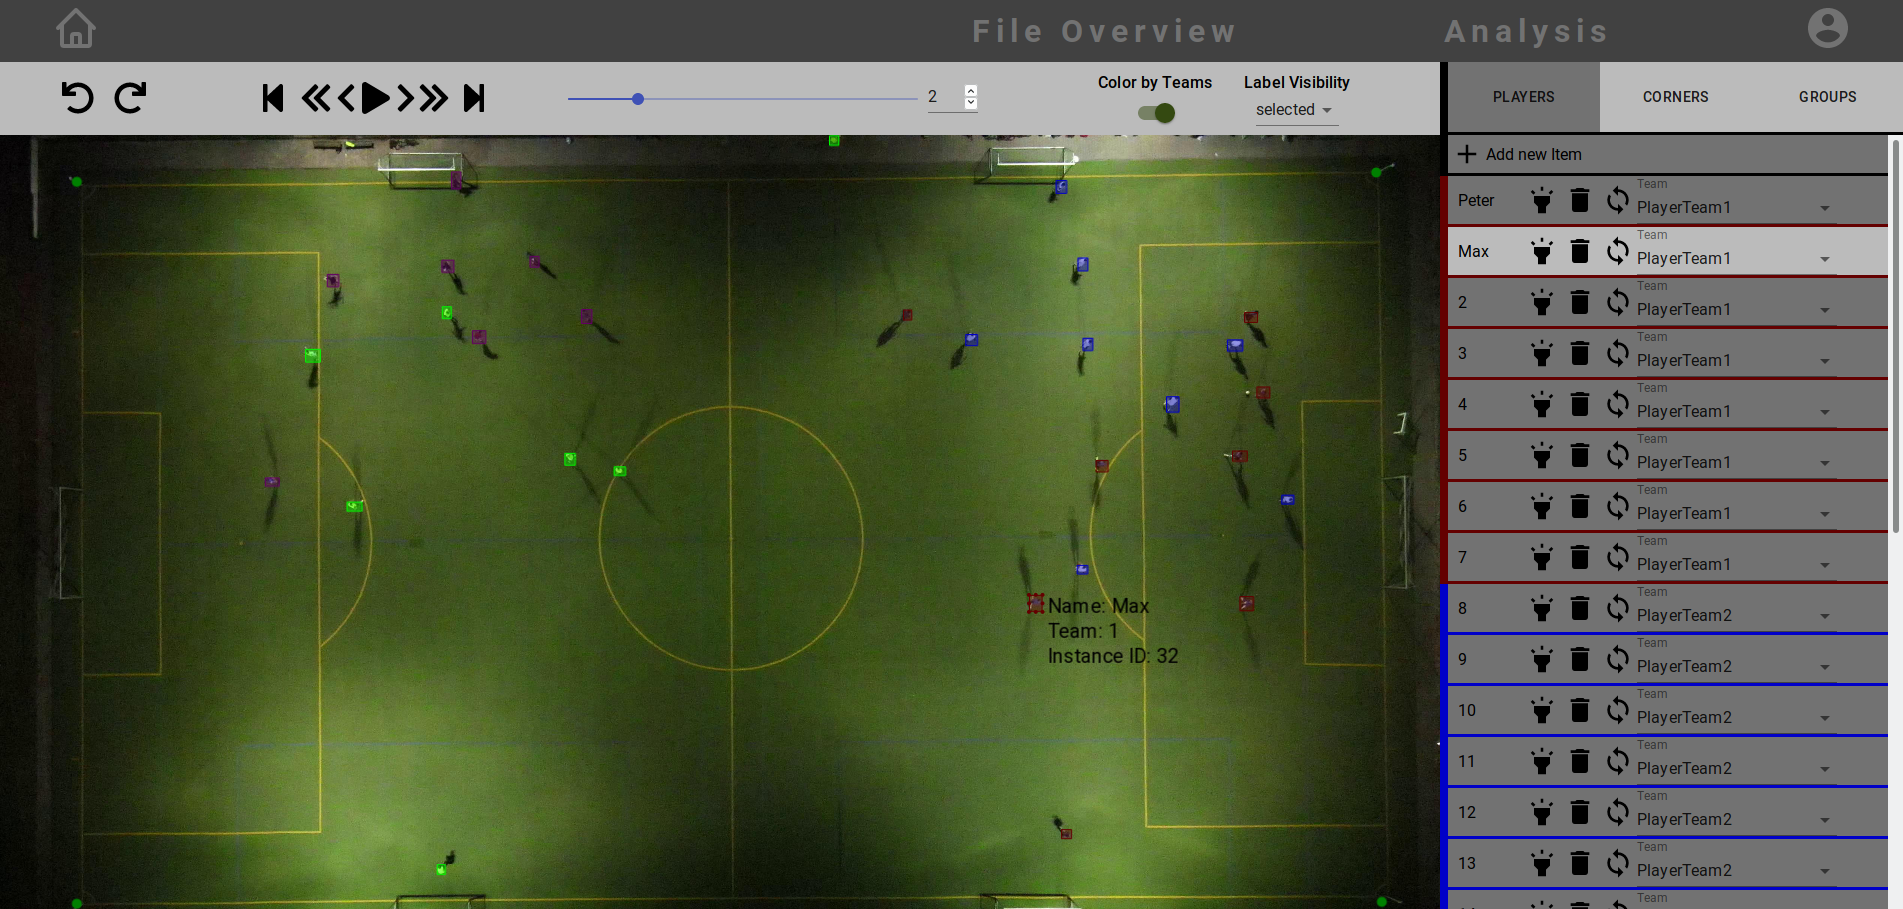
\includegraphics[width=17cm]{images/Tracking_Editor.png}
 \caption{Die Tracking Editor Seite.}
 \label{fig:tracking-editor}
\end{figure}


Die gesamte Logik für die Ausführung all dieser Funktionen befindet sich in der \texttt{TrackingEditor} Komponente. State Variablen werden bei React immer so tief wie möglich, also sprich immer möglichst im Kindkomponent verwaltet. Allerdings sind auf dieser Seite immer mehrere Komponenten vom State abhängig, weswegen dieser zum Großteil gesammelt in der hierarchisch obersten Komponente \texttt{TrackingEditor} verwaltet wird. Die Kindkomponenten rufen Funktionen des Vaters auf, der dann durch seine state Änderung sich und seine Kinder mit den aktualisierten Daten erneut rendert. Beispielsweise wird der aktuelle Frame in der \texttt{Navbar} gewählt, von dort wird allerdings nur eine Funktion in \texttt{TrackingEditor} aufgerufen, da dort der aktuelle Frame verwaltet wird, da bei einer Änderung die \texttt{Navbar}, das Hintergrundbild des Canvas im \texttt{TrackingEditor}, sowie die in der \texttt{TrackList} angezeigten Trackingdaten upgedatet werden müssen. Auch die einzelnen Kinder der \texttt{TrackList} Komponente werden nicht von dieser, sondern direkt von \texttt{TrackingEditor} erzeugt und als Props an das Kind \texttt{TrackList} übergeben und dort angezeigt. \\
\\
Generell wird in React das Aussehen der Komponenten und damit der Website über die state Variable (bzw. die Props) geregelt und Änderungen dieser werden automatisch erkannt und führen zu einem Rerender der Komponenten, in denen sich etwas verändert hat. Das Fabric Canvas Element passt allerdings nicht in dieses Schema, da dort nur tief verschachtelte Elemente verändert werden, was von React nicht unterstützt/erkannt wird. Fabric bzw. der Programmierer selbst ist für das Rerendering des Canvas zuständig, weshalb es auch ohne ein Rerender der React Komponente, in der es eingebettet ist, aktualisiert werden kann. Der resultierende Code entspricht dann allerdings nicht den React Prinzipien und Standards, da die Konzepte der Bibliotheken sich gegenseitig widersprechen. JS ermöglicht es nicht, beliebig verschachtelte Objekte zu kopieren und dann zu verändern und bei React dürfen die state Variablen nicht direkt verändert werden, da dann der Abgleich der alten und neuen Werte nicht mehr funktioniert und die Änderung nicht erkannt wird. Bibliotheken wie z.B. immutability-helper (\url{https://github.com/kolodny/immutability-helper}) können hier ebenfalls nur bis zu einem gewissen Grad Abhilfe schaffen. Nach einigen Problemen mit der gemeinsamen Verwendung wurde folgende Lösung gefunden: Die Canvas Elemente werden nicht im state verwaltet, aber falls sie sich auf eine Weise verändern, die ein Rerender von React Komponenten (z.B. der TrackList) notwendig machen, wird eine Dummy Boolean Variable im state negiert, um diesen Rerender auszulösen. Dies macht es außerdem möglich, die einzelnen Bounding Boxes direkt als Props bzw. Parameter an Kindkomponenten zu übergeben und bei notwendigen Änderung sie wiederum von den Kindkomponenten an die jeweiligen Funktionen in \texttt{TrackingEditor} als Parameter zu übergeben, wo diese direkt verändert werden können, ohne erst den state nach Ihnen zu durchsuchen. Meiner Meinung nach ist dies die mit den aktuellen Möglichkeiten von React sinnvollste Möglichkeit, die Canvas Elemente zu verwalten und macht viele Operationen, die React klassischerweise bedingen würde (state nach passender Variable/Key/Bounding Box durchsuchen sowie Kopieren, ändern und updaten der passenden state Variable, um deren immutability nicht zu verletzen) überflüssig. \\
\\
Da in \texttt{TrackingEditor} die meisten Daten verwaltet werden, sind hier auch die meisten für das Backend wichtigen Infos zu finden. Wie in allen anderen Komponenten wurde im Code an jeder relevanten Stelle ein erklärender und mit ``TODO BACKEND'' versehener Kommentar eingefügt. Zusätzlich steht hinter jeder state Variable, die zukünftig vom Backend verwaltet werden soll, ein ``BACKEND'' Kommentar. Diese Variablen sollten wohl am besten an den im Code gekennzeichneten Stellen Daten vom Backend abrufen und diese dann weiterhin im state speichern, damit die Komponenten mit geänderten Daten erneut von React gerendert werden. \\

Bei Beginn der Implementierung wurde ein Cache entworfen, der eine im Code festlegbare Anzahl an Frames lädt, um diese dann bei Bedarf direkt anzuzeigen. Allerdings hat sich relativ früh herausgestellt, dass ein einzelnes Laden der lokalen Videoframe Bilddateien besser und zuverlässiger funktioniert. Der Code für den Cache wurde allerdings im Code belassen und mit einigen Kommentaren zu Funktionsweise und Weiterentwicklung ergänzt. Bei Vorhandensein eines Backends wäre es meiner Meinung nach vielversprechend, diese Funktion weiterzuentwickeln und weiter damit zu experimentieren. Zum Beispiel könnte, falls gerade keine anderen Daten vom Backend geladen werden, dieses automatisch bereits den oder die nächsten Frames senden. So könnte, sobald der Nutzer einen Frame weiterspringt, dieser mit deutlich weniger Wartezeit angezeigt werden, was die Webapp insgesamt deutlich reaktiver und schneller machen könnte. Zusätzlich könnte die Auflösung der Bilder angepasst werden, oder sogar erst ein weniger stark aufgelöstet Bild angezeigt werden und anschließend der Frame in voller Auflösung geladen werden. Solche Überlegungen setzen allerdings weitere Tests mit Backend voraus, um zu evaluieren, inwiefern diese notwendig sind.







\subsection{Analyse}\label{chapter:analysis}

Nachdem der Nutzer die Trackingdaten überprüft und gegebenenfalls korrigiert hat, steht das Erstellen einer Spielanalyse an. Dazu dient die sich an der URL \texttt{/analysis/<game\_id>} befindende Analyse Seite, die in \autoref{fig:analysis-1} und \ref{fig:analysis-2} zu sehen ist. \\

\begin{figure}[!h]
 \centering
 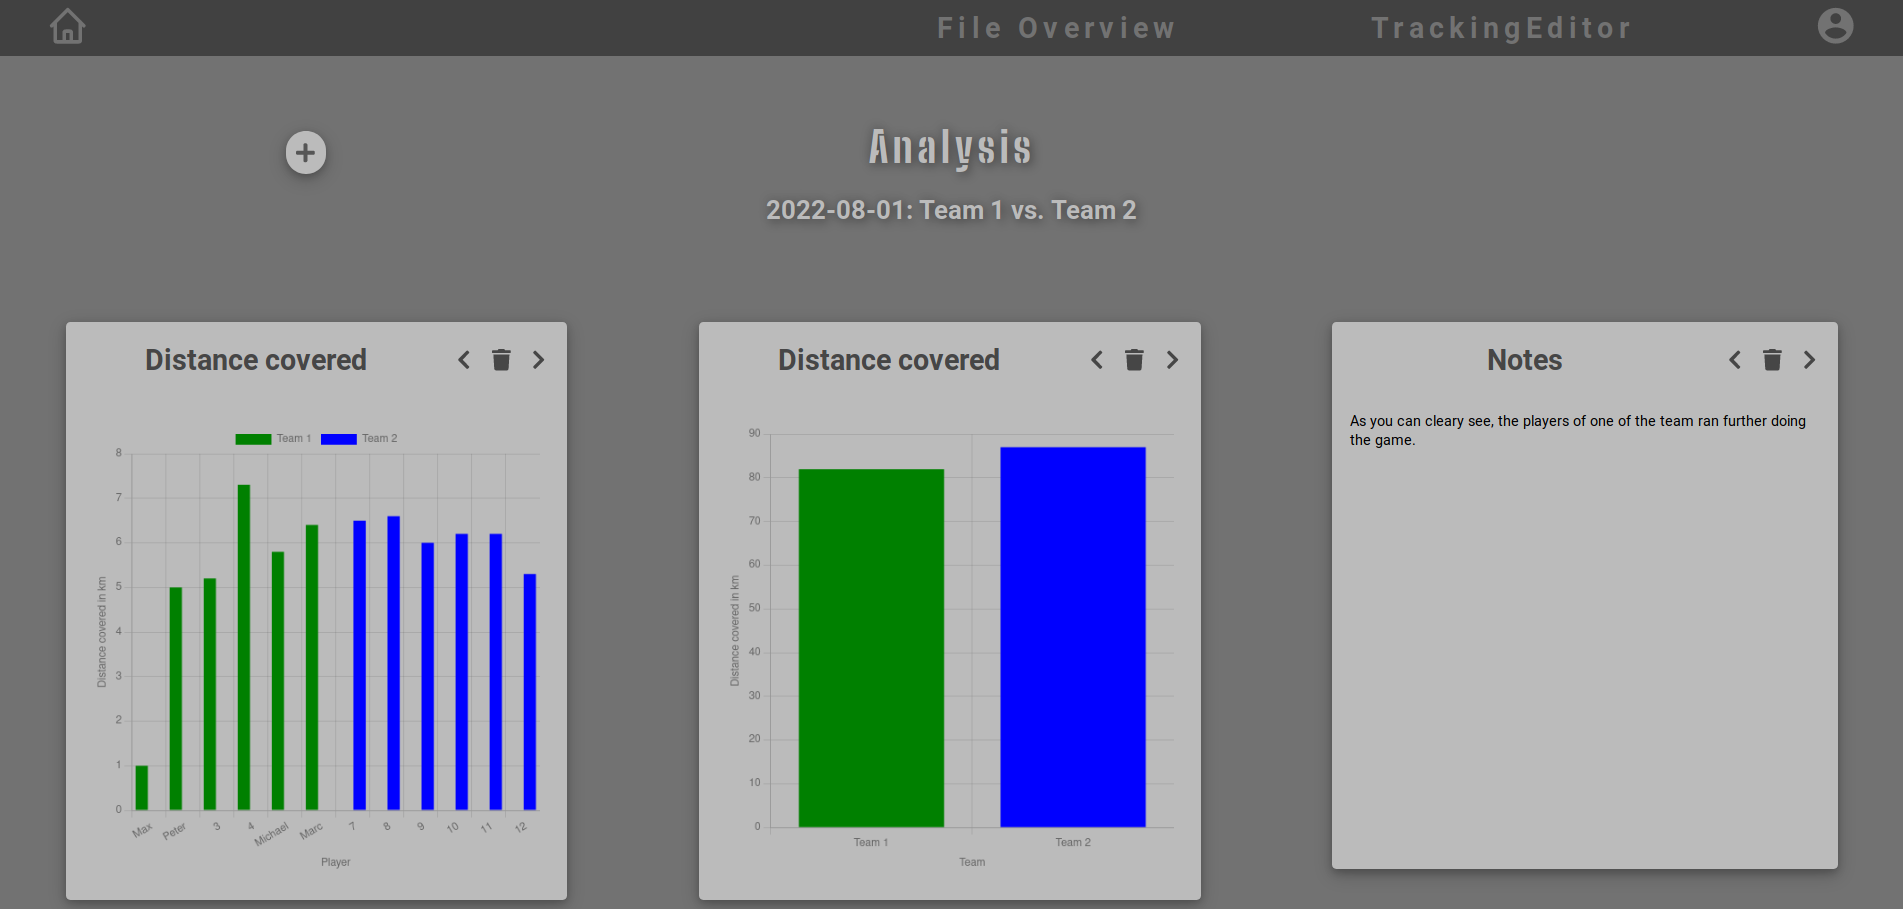
\includegraphics[width=17cm]{images/Analysis_1.png}
 \caption{Die Analyse Seite mit zwei unterschiedlich konfigurierten Barchart Tiles und einem Notiz Tile.}
 \label{fig:analysis-1}
\end{figure}

\begin{figure}[!h]
 \centering
 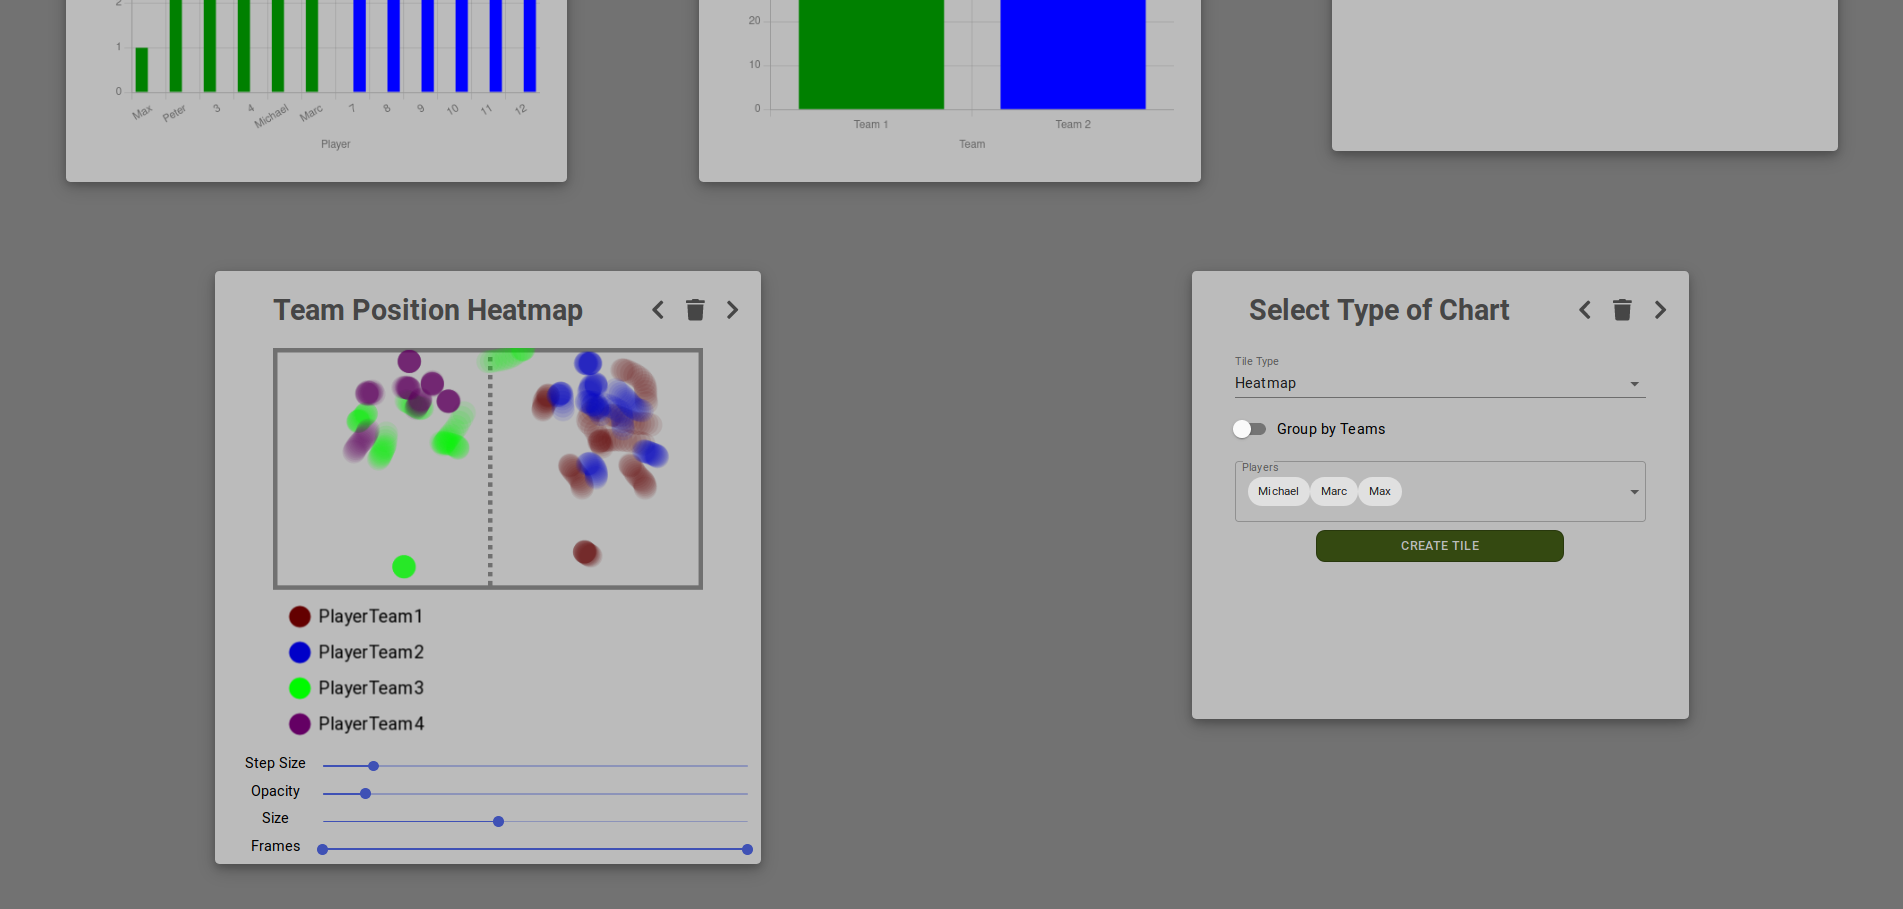
\includegraphics[width=17cm]{images/Analysis_2.png}
 \caption{Der untere Teil der Analyse Seite mit einem Heatmap Tile und einem TileTypeSelector Tile mit einigen bereits erfolgten Einstellungen zur Erstellung eines neuen Tiles.}
 \label{fig:analysis-2}
\end{figure}

% Added space in long path below for line break: \texttt{/src/components/ pages/analysis/}
Die gesamte Seite (bis auf die \texttt{Header} Komponente wie auch bei allen anderen Seiten) ist in der \texttt{Analysis} Komponente beschrieben, die in der gleichnamigen JS Datei im Ordner \texttt{/src/components/ pages/analysis/} zu finden ist. Dort werden dann die entsprechenden Kindkomponenten eingefügt. Die hellgrauen Kästen, die alle jeweils eine Art der Analyse bzw. ein Diagramm enthalten, sind \texttt{AnalysisTile} Komponenten. \texttt{Analyis} verwaltet im state die Einstellungen aller Analyse Tiles. Es werden nur die Parameter gespeichert, mit denen die tatsächlich anzuzeigenden Daten für die einzelnen Diagramme oder Heatmaps vom Backend abgerufen werden können. Nur für die Notiz Tiles, die nur einen vom Nutzer eingegebenen Text anzeigen, wird dieser direkt gespeichert. So wird sichergestellt, dass alle anderen Tiles immer die aktuellste Version der Daten vom Backend abrufen und keine Duplizierung der Daten stattfindet. Die einzelnen Tiles können mit den Buttons in der rechten oberen Ecke in der Reihenfolge verändert (mit dem linken oder rechten Nachbarn vertauscht) und gelöscht werden. Die Reihenfolge der Tiles wird in der \texttt{order} Variable im state der \texttt{Analysis} Komponente in Form einer Liste der Ids der einzelnen \texttt{AnalysisTile} Komponenten gespeichert. Die Einstellungen/Metadaten jedes einzelnen Tiles sind in der state Variable \texttt{analysisTiles} als Liste gespeichert. Solange kein Backend integriert ist, werden diese aus der Klassenvariable \texttt{defaultAnalysisTiles} geladen, die einige Beispielanalysen bereitstellt. Sobald ein Backend vorhanden ist, muss dieses aufgerufen werden um die evtl. bereits erstellten Analyse Tiles zu laden und bei Schließen der Analyse zu speichern. Die notwendigen Änderungen wurden wieder im Code genau beschrieben und mit ``TODO BACKEND'' Kommentaren versehen.\\
Die Reihenfolge der Tiles wird mithilfe des \texttt{order} CSS Props definiert. Diese ändert die Reihenfolge, in der die Elemente in einem Flexbox (oder Grid) Container angezeigt werden. So wird die Anzeigereihenfolge von den Metadaten entkoppelt und die Tiles bleiben in der Liste \texttt{defaultAnalysisTiles} immer nach Id geordnet (da die Id eines gelöschten Tiles nicht noch einmal verwendet wird).\\
\\
Die Metadaten für jeden \texttt{AnalysisTile} sowie dessen Typ (also die Art der anzuzeigenden Analyse/Diagramms) werden direkt an diesen Übergeben und dort werden dann gegebenenfalls die von den aktuellen Trackingdaten abhängigen Daten aus dem Backend geladen. Momentan werden diese Daten statt aus dem Backend aus einigen in \texttt{/src/data/} abgelegten JSON Dateien geladen, deren Name immer mit ``analysis\_'' beginnt. Diese sind im Prinzip Beispielantworten des späteren Backends und zeigen genau das für die einzelnen Typen von Tiles notwendige Format. Wo genau diese Anfragen im Code gestellt und weiterverarbeitet werden müssen, ist mit den üblichen Kommentaren gekennzeichnet.\\

Um das Hinzufügen neuer Arten von Analysen zu vereinfachen, existiert in \texttt{AnalysisTile} neben den Props für die ausgewählten Teams und/oder Spieler auch ein generischer \texttt{tileState} Prop, der momentan z.B. bereits für die Heatmap verwendet wird. Jede \texttt{AnalysisTile} Komponente erzeugt dann aus diesen übergebenen Daten bzw. auf Grundlage der mit Hilfe dieser Daten aus dem Backend abgefragten Daten seinen Inhalt. Die momentan unterstützen Tiles sind Notiz, Balkendiagramm, Heatmap und Konfigurations-Tile (im Code TileTypeSelector genannt), die alle in \autoref{fig:analysis-1} und \ref{fig:analysis-2} zu sehen sind. Notizen werden direkt erzeugt, für alle anderen Arten wird eine weitere Kindkomponente \texttt{BarChart}, \texttt{Heatmap} oder \texttt{TileTypeSelector} aus den vorliegenden Daten erzeugt und im \texttt{AnalysisTile} angezeigt. Die \texttt{BarChart} Komponente wurde möglichst generisch gelassen, was sich auch daran zeigt, dass die ersten beiden in \autoref{fig:analysis-1} zu sehenden Tiles diese beide benutzen und sich nur in den vom Backend empfangenen bzw. momentan noch aus einer lokalen Datei ausgelesen Daten unterscheiden. Auch die Beschriftungen der Achsen sind nicht im Code sondern in den dem Diagramm zu Grunde liegenden Daten festgelegt. So kann sehr leicht eine neue Art von Balkendiagramm integriert werden, z.B. für den Ballbesitz oder die Anzahl der Torschüsse, sobald das Backend dies unterstützen sollte. Dafür müsste nur in \texttt{AnalysisTile} ein neue Art von Diagramm unterstützt werden, die genau wie ``distance-barchart'' eine \texttt{BarChart} Komponente mit den Daten des Backends erstellt und den Titel des Tiles passend setzt (also die Variable \texttt{headingText} in der \texttt{render()} Funktion). Außerdem muss dieser Tile Typ sowie alle gewünschten Auswahlmöglichkeiten für diesen Typ in der \texttt{TileTypeSelector} Komponente analog zu ``distance-barchart'' ergänzt werden.\\
\\
Genau wie für die \texttt{FileOverview} Komponente wurde auch bei der Analyse Seite der alternative Hintergrund getestet, der in \autoref{fig:analysis-alternative-background} zu sehen ist. Auch hier habe ich mich dann allerdings für den auf den vorherigen Abbildungen verwendeten Standardhintergrund entschieden, um die eigentlichen Inhalte der Analysen mehr in den Vordergrund zu stellen. Allerdings wurde wieder der Code für den texturierten Hintergrund in der CSS Datei für die Analyse Seite belassen und dieser kann wieder aktiviert werden, wie durch den ``GRASS BACKGROUND'' Kommentar im Code beschrieben.


\begin{figure}[h]
 \centering
 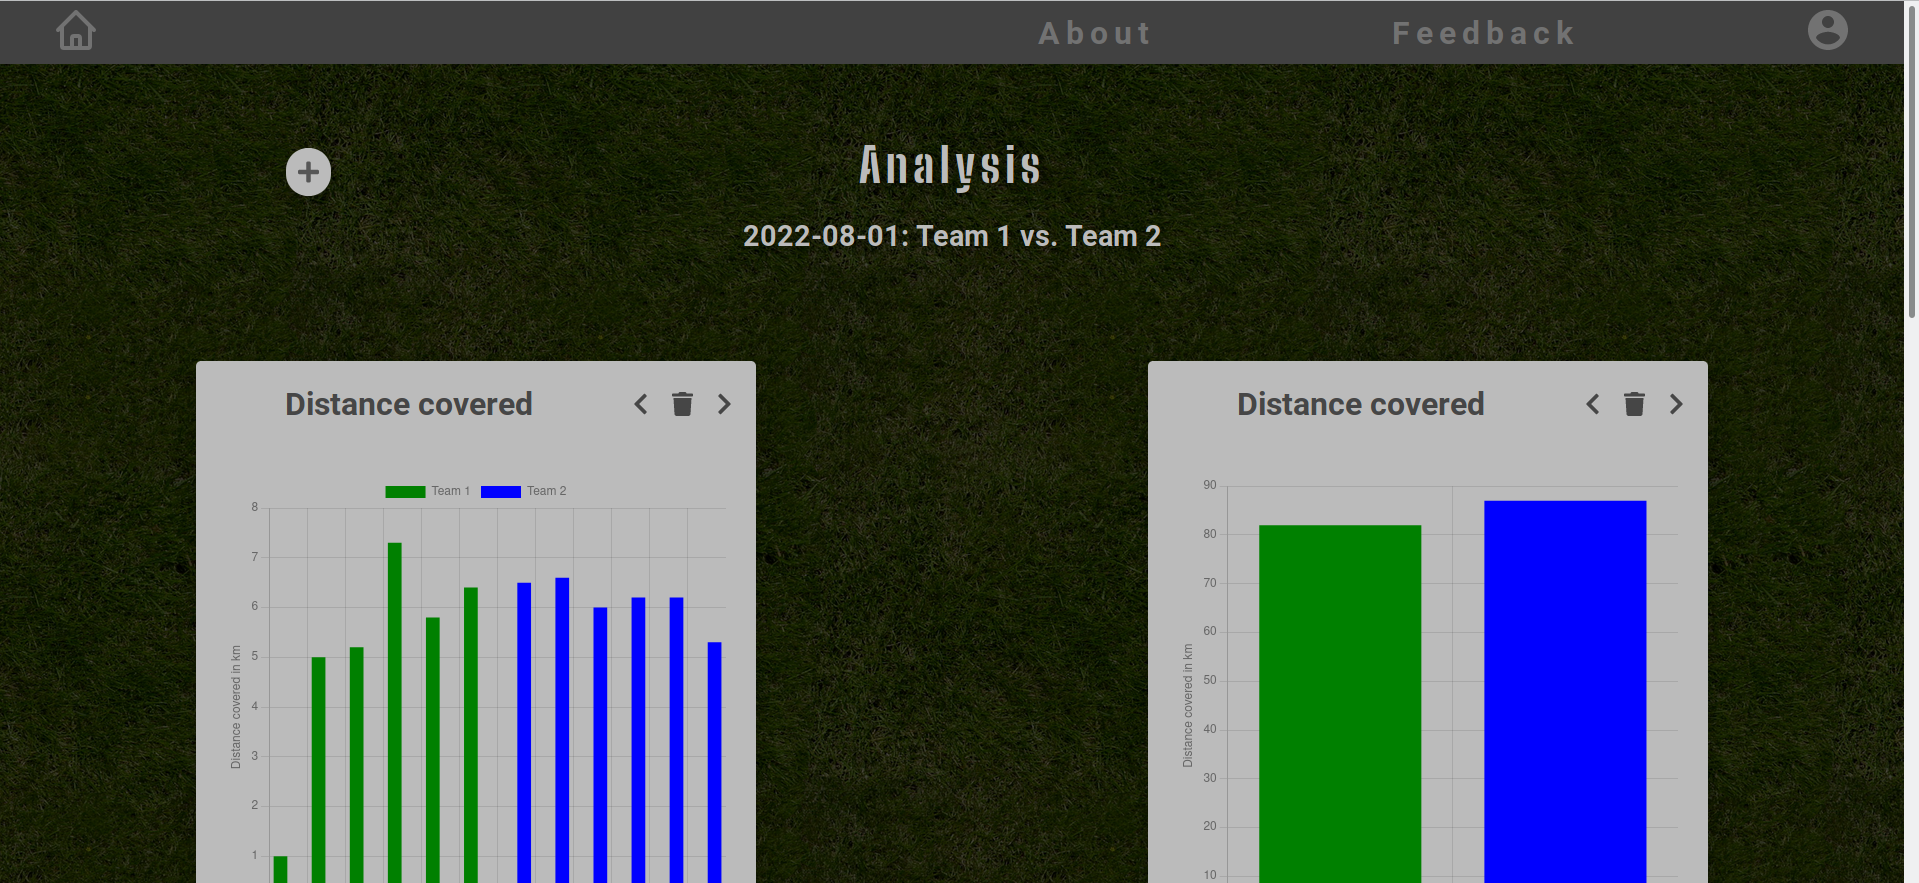
\includegraphics[width=17cm]{images/Analysis_with_grass_background.png}
 \caption{Die Analyse Seite mit dem alternativen Grashintergrund.}
 \label{fig:analysis-alternative-background}
\end{figure}